\documentclass[18 pt]{beamer}
\usetheme{Madrid}
% \usefonttheme{professionalfonts}
\usefonttheme{structurebold}
\usecolortheme{rose}
\setbeamerfont{title}{size=\LARGE, series=\bfseries}
% \setbeamerfont{subtitle}{size=\large}
% \setbeamerfont{author}{size=\large}
% \setbeamerfont{date}{size=\large}
% \setbeamerfont{frametitle}{size=\Large, series=\bfseries}
% \setbeamerfont{framesubtitle}{size=\large}
% \setbeamerfont{normal text}{size=\huge}
\usepackage{enumitem}

\setlist[enumerate]{label={}, leftmargin=*,itemsep=15pt}
\setbeamerfont{enumerate item}{size=\LARGE}

\usepackage{amsmath}
\usepackage{amssymb}
\usepackage{listings}
\usepackage{booktabs}
\usepackage{multirow}
\usepackage{multirow}
\usepackage{lmodern}
\usepackage{xcolor}
\usepackage{float}
\lstset{
  language=Python,  %代码语言使用的是matlab
  % frame=shadowbox, %把代码用带有阴影的框圈起来
  rulesepcolor=\color{red!20!green!20!blue!20},%代码块边框为淡青色
  keywordstyle=\color{blue!90}\bfseries, %代码关键字的颜色为蓝色,粗体
  commentstyle=\color{red!10!green!70}\textit,    % 设置代码注释的颜色
  basicstyle=\footnotesize,
  showstringspaces=true,%不显示代码字符串中间的空格标记
  % numbers=left, % 显示行号
  % numberstyle=8pt,    % 行号字体
  % numberstyle=\color{green},
  stringstyle=\rmfamily\slshape\color[RGB]{128,0,0}, % 代码字符串的特殊格式
  breaklines=true, %对过长的代码自动换行
  extendedchars=false,  %解决代码跨页时,章节标题,页眉等汉字不显示的问题
  escapeinside=``,%代码中出现中文必须加上,否则报错
  texcl=true}

\lstset{breaklines}%自动将长的代码行换行排版

\lstset{extendedchars=false}%解决代码跨页时,章节标题,页眉等汉字不显示的问题

\usepackage{textcomp}
% \usepackage[margin=1in]{geometry}
\usepackage{pythonhighlight}
% \usepackage{minted}
\usepackage[backend=bibtex]{biblatex}
%\usepackage[style=authortitle,backend=biber]{biblatex}
\addbibresource{ResearchRabbit_Export_2022_10_20.bib}

\usepackage{algorithm}
\usepackage{algorithmic}
\renewcommand{\algorithmicrequire}{\textbf{Input:}}
\renewcommand{\algorithmicensure}{\textbf{Output:}}


\title{Copyright in QDA }
\author[Gcc]{Dingchao Gao}
\institute[ISCAS]{Institute of Software Chinese Academy of Sciences}

\setbeamertemplate{footline}[frame number]
\begin{document}

\begin{frame}[plain]
  \titlepage
\end{frame}

\section{References}
\begin{frame}[noframenumbering,allowframebreaks,t]
	\frametitle{references}
  \nocite{*}
  \printbibliography
\end{frame}

\begin{frame}
  \begin{figure}
    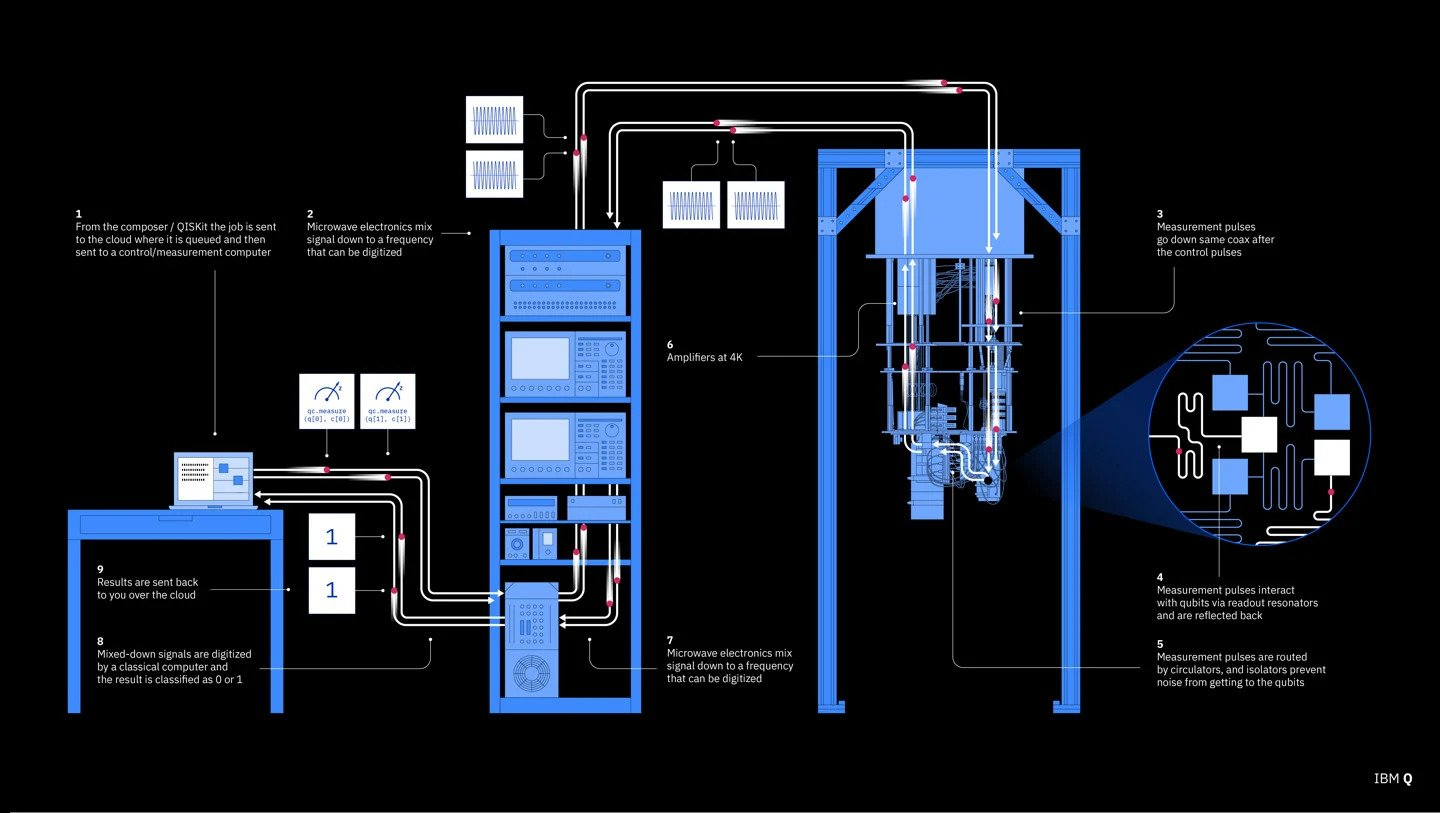
\includegraphics[width =\textwidth]{IBM.jpg}
  \end{figure}
\end{frame}

% 问题
% 重要性
% 前人工作
% methodology + innovation
% 预期结果
% \begin{frame}
%   \begin{figure}
%   \end{figure}
% \end{frame}
\begin{frame}
  \begin{frame}
    \begin{center}
    \begin{tikzpicture}[node distance=2cm]
    \node (start) [circle, draw] {Start};
    \node (process1) [rectangle, draw, below of=start] {Process 1};
    \node (decision) [diamond, draw, below of=process1] {Decision};
    \node (process2a) [rectangle, draw, below left of=decision] {Process 2a};
    \node (process2b) [rectangle, draw, below right of=decision] {Process 2b};
    \node (end) [circle, draw, below of=decision] {End};
    
    \draw [->] (start) -- (process1);
    \draw [->] (process1) -- (decision);
    \draw [->] (decision) -- node[anchor=east] {Yes} (process2a);
    \draw [->] (decision) -- node[anchor=west] {No} (process2b);
    \draw [->] (process2a) -- (end);
    \draw [->] (process2b) -- (end);
    \end{tikzpicture}
    \end{center}
\end{frame}
\end{document}